In this section, we analyze the scalability of several LM programs using up to
32 threads. We also compare the run times against the run time of the
hand-written C++ programs when such run times are available. We used the
programs of the previous section with a few additions:

\begin{itemize}

      \item PageRank: an asynchronous version of the PageRank program without
         synchronization between iterations. Every time a node sends a new
         PageRank value to its neighbors and the change is significant, then the
         neighbors are scheduled to recompute their PageRanks.

      \item Greedy Graph Coloring~(GGC): an algorithm that colors nodes in a
         graph so that no two adjacent nodes have the same color. We start with
         a small number of colors and then we expand the number of colors when
         we cannot color the graph.

\end{itemize}

We executed all the programs using 17 configurations: the first uses 1 thread
and the other 16 use even numbers of threads for a maximum of 32 threads. In the
plots presented next, the bottom axis represents the number of threads used when
executing the program, the left axis represents the run time (in milliseconds)
for that particular configuration and the right axis represents the speedup
computed using $T_1/T_i$, where $i$ represents the number of threads and
$T_x$ the run time of the program using $x$ threads.  In some plots, there is
also an horizontal black line that represents the run time of the C++ program
and is used to understand how many threads are needed in order for an LM program
to run faster than the C++ program. Note that all the run times are the average
of three runs.

\newcommand{\plotsize}[0]{0.4}

The scalability results for the Belief Propagation program are presented in
Fig.~\ref{fig:implementation:scale_bp}. This program has the best scalability
with a 60-fold speedup for 32 threads. This is because the default ordering used
for 1 thread leads to a slow convergence rate, resulting in super-linear
speedups. When using multiple threads, the graph will converge faster, because
belief updates have more up-to-date information from neighbor nodes due to the
existence of multiple threads.  Note that we also used the same computation
ordering in the C++ program, which is also the one used in the GraphLab
framework.

\begin{figure}[]
        \centering
        \begin{subfigure}[b]{\plotsize\textwidth}
                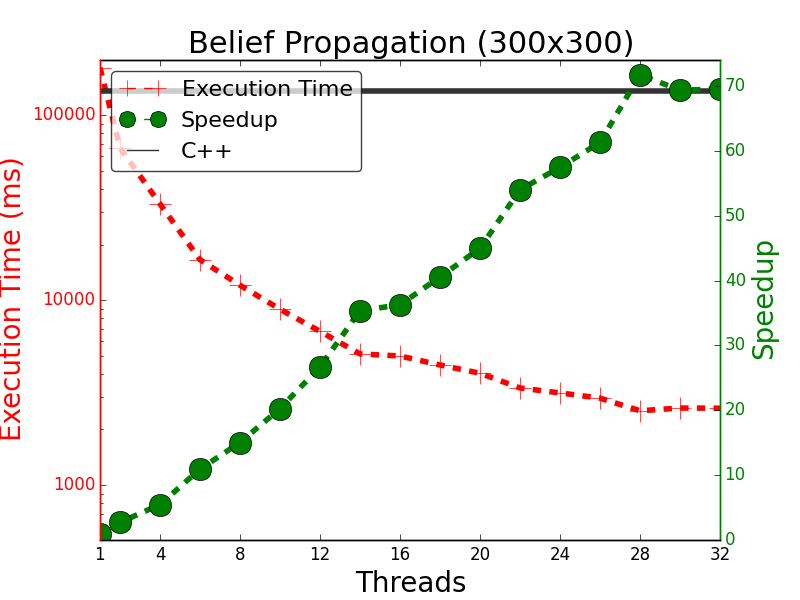
\includegraphics[width=\textwidth]{experiments/scalability/scale-belief-propagation-300.png}
                \label{fig:implementation:scale_bp300}
        \end{subfigure}
        ~
        \begin{subfigure}[b]{\plotsize\textwidth}
                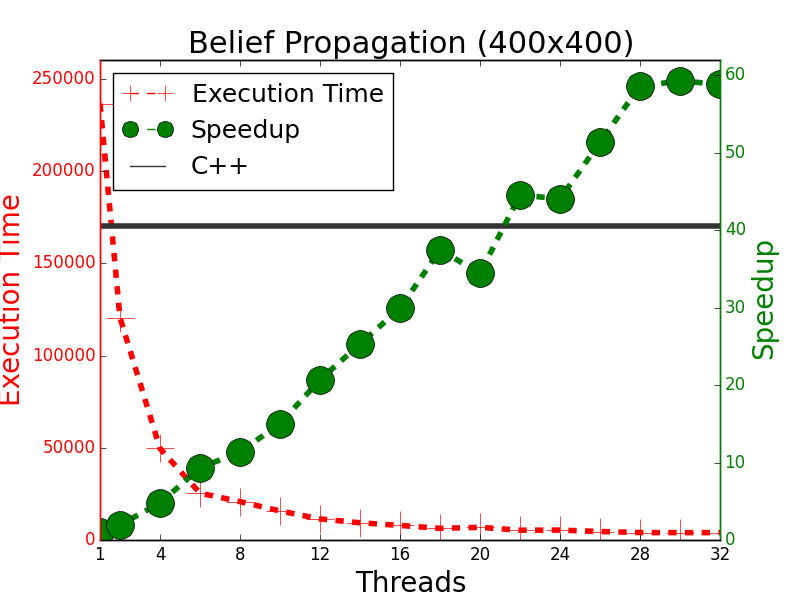
\includegraphics[width=\textwidth]{experiments/scalability/scale-belief-propagation-400.png}
                \label{fig:implementation:scale_bp400}
        \end{subfigure}\\
        \caption{Scalability results of the Belief Propagation program. The
        super-linear speedup is a consequence of the existence of multiple
        threads, which allows the program to converge faster.}
        \label{fig:implementation:scale_bp}
\end{figure}

The results for the Heat Transfer program are shown in
Fig.~\ref{fig:implementation:scale_ht}. We note that LM requires around 15
threads to reach the run time of the C++ program. This results from the poor
absolute performance of the LM program that was mentioned in the previous section.
Although we use a grid dataset, the work available in the graph is not equally
distributed due to different initial heat values, therefore an almost linear
speedup should not be expected. When comparing the two datasets used, the 80x80
configuration has less scalability than the 120x120 dataset due to its smaller
size. For the 120x120 dataset, LM has a 12-fold speedup for 32 threads, which
makes the LM version run almost twice as fast as the C++ version.

\begin{figure}[]
        \begin{subfigure}[b]{\plotsize\textwidth}
                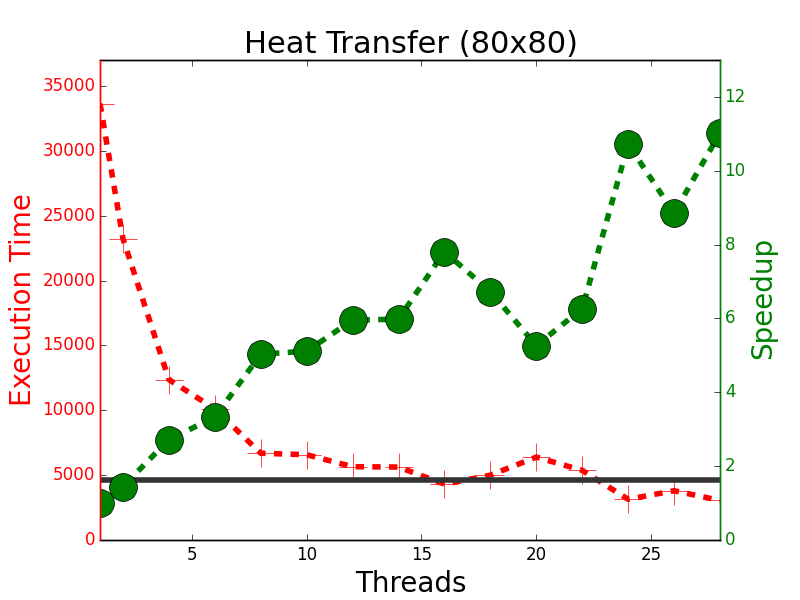
\includegraphics[width=\textwidth]{experiments/scalability/scale-new-heat-transfer-80.png}
                \label{fig:implementation:scale_ht80}
        \end{subfigure}
        ~
        \begin{subfigure}[b]{\plotsize\textwidth}
                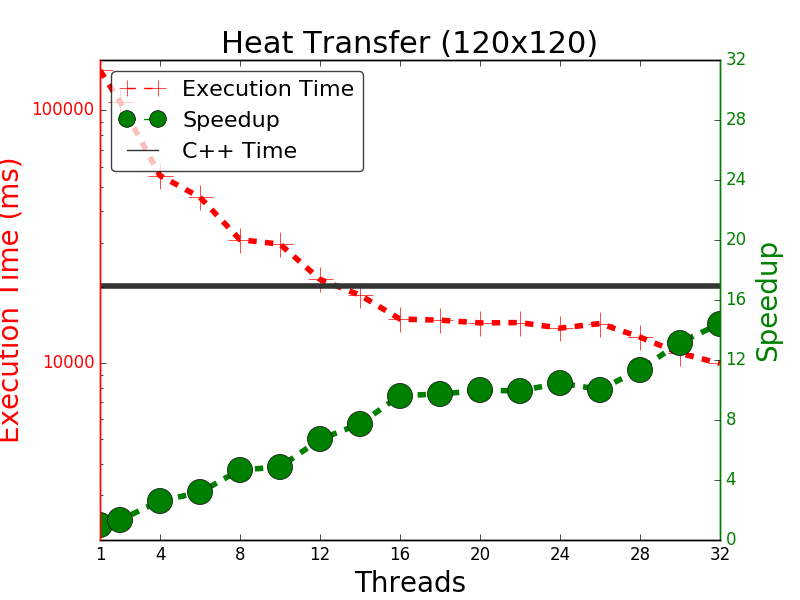
\includegraphics[width=\textwidth]{experiments/scalability/scale-new-heat-transfer-120.png}
                \label{fig:implementation:scale_ht120}
        \end{subfigure}\\
        \caption{Scalability results for the Heat Transfer program. Because the
           Heat Transfer program performs poorly when compared to the C++ program,
           the LM version needs at least 15 threads to reach the run time of the C++
           program.}
        \label{fig:implementation:scale_ht}
\end{figure}

Figure~\ref{fig:implementation:scale_ggc} presents the results for the Greedy
Graph Coloring~(GGC) program. In GGC, we use two datasets: Google
Plus~\cite{snapnets}, a graph representing social circles in Google Plus with
107614 nodes and 13673453 edges, and Twitter, a graph representing Twitter
networks with 81306 nodes and 1768149 edges (note that Twitter was also used
before in the MSSD program).  Since Twitter is a much smaller dataset, its
speedup is much smaller than Google Plus, as expected. However, while the
speedup of Twitter starts to drop after 16 threads, the LM system is still able
to make it faster by adding more threads. For Google Plus, a 20-fold speedup is
achieved for 32 threads, which is a reasonable scalability considering that GGC
is not a program where work is equally distributed.

\begin{figure}[]
        \begin{subfigure}[b]{\plotsize\textwidth}
                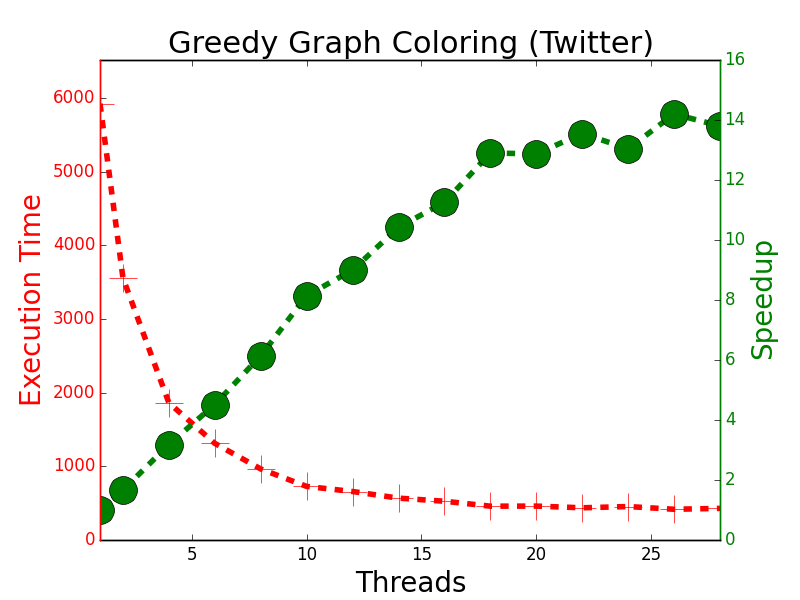
\includegraphics[width=\textwidth]{experiments/scalability/scale-greedy-graph-coloring-twitter.png}
                \label{fig:implementation:scale_ggc_twitter}
        \end{subfigure}
        ~
        \begin{subfigure}[b]{\plotsize\textwidth}
                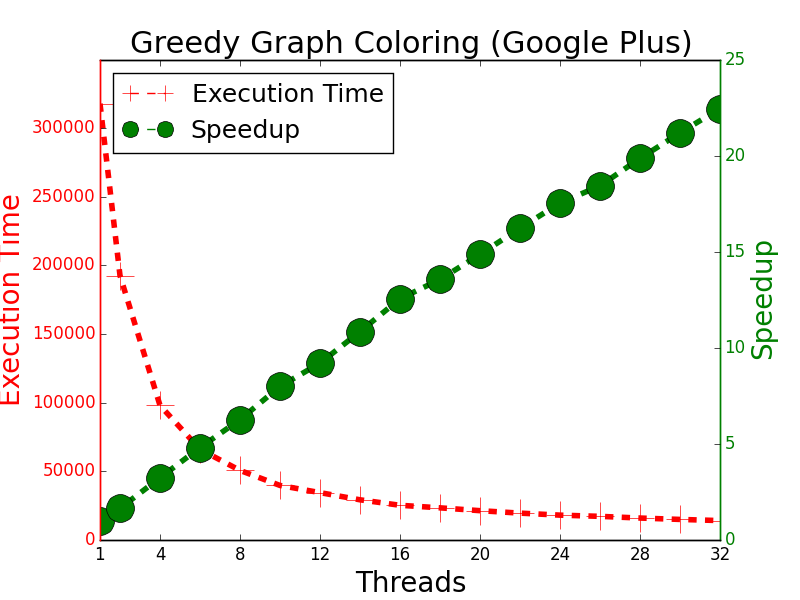
\includegraphics[width=\textwidth]{experiments/scalability/scale-greedy-graph-coloring-gplus.png}
                \label{fig:implementation:scale_ggc_gplus}
        \end{subfigure}\\
        \caption{Scalability of the Greedy Graph Coloring program. The Twitter
           and Google Plus datasets have almost the same number of nodes but
           Google Plus has ten times more edges, which makes coloring more time
           consuming.}
        \label{fig:implementation:scale_ggc}
\end{figure}

The results for the N-Queens program are shown in
Fig.~\ref{fig:implementation:scale_queens}. We decided to just use the 13 and 14
configurations since those take longer to run. The 13-Queens configuration has
169 nodes while the 14-Queens configuration has 196 nodes. The LM program
considers the chess board as a graph and the bottom rows have more work to
perform since the valid queens placements are built from the top to the bottom
row. For a more in-depth explanation of the N-Queens program please see
Section~\ref{section:coord:nqueens}.

Due to the small number of nodes in the N-Queens program and the fact that more
work is performed at the bottom rows, the N-Queens program is hard to
parallelize. Furthermore, the solutions for the puzzle are built by constructing
lists which are shared between threads. This introduces some potential false
sharing because the reference count of each list data structure needs to be
updated when new solutions are constructed. The 14-Queens configuration has good
efficiency using 16 to 20 threads, while the 13-Queens configuration efficiency
starts to drop after 14 threads. One can argue that the best number of threads
is correlated to the size of the board, because the second half of execution is
better balanced and partitioned when the number of threads matches the size of
the board.

\begin{figure}[]
        \centering
        \begin{subfigure}[b]{\plotsize\textwidth}
                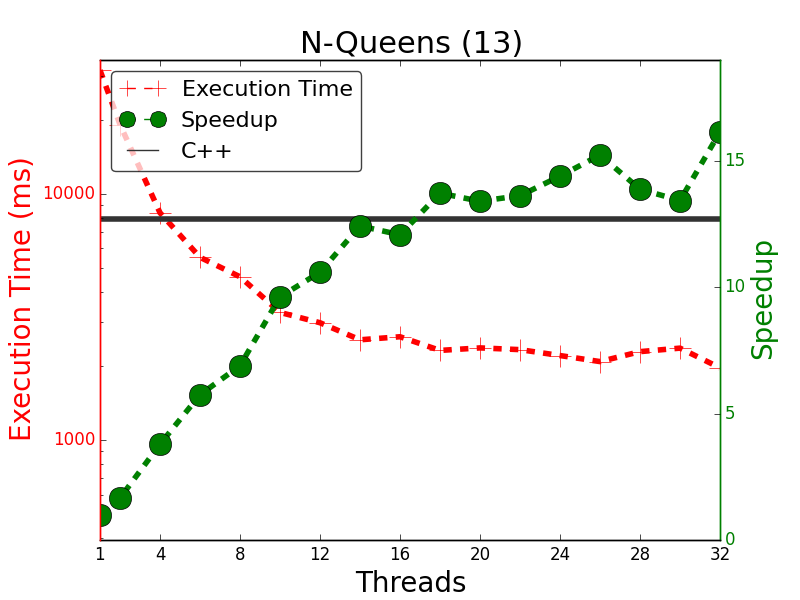
\includegraphics[width=\textwidth]{experiments/scalability/scale-8queens-13.png}
                \label{fig:implementation:scale_queens13}
        \end{subfigure}
        ~
        \begin{subfigure}[b]{\plotsize\textwidth}
                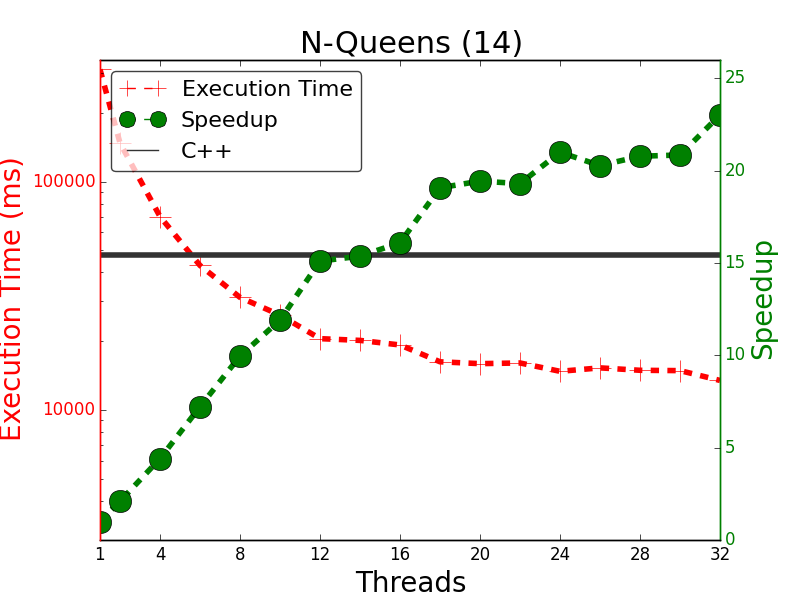
\includegraphics[width=\textwidth]{experiments/scalability/scale-8queens-14.png}
                \label{fig:implementation:scale_queens14}
        \end{subfigure}

        \caption{Scalability results for the N-Queens program. The 13
        configuration has 73712 solutions, while the 14 configuration has 365596
     solutions. In terms of graph size, the 13 configuration has $13 \times 13$
  nodes while the 14 configuration has $14 \times 14$ nodes.}

        \label{fig:implementation:scale_queens}
\end{figure}

The speedup results for the MiniMax program is shown in
Fig.~\ref{fig:implementation:scale_minmax}.  This is an interesting program
because the graph is constructed during run time. Furthermore, due to the LM
default scheduling order, the tree is explored in a breadth-first fashion,
requiring the program to hold the complete MiniMax tree in memory. The Big
configuration, for instance, uses, on average, 14GB of memory and a total of
30GB of memory before collecting the tree. Since the machine used for the
experiments has only 32GB, the Small configuration scales better due to the
smaller memory requirements. In Section~\ref{section:coord:minimax}, we will
show how this program can be improved by changing the default scheduling order
of LM and improving the memory usage of the program.

\begin{figure}[]
        \begin{subfigure}[b]{\plotsize\textwidth}
                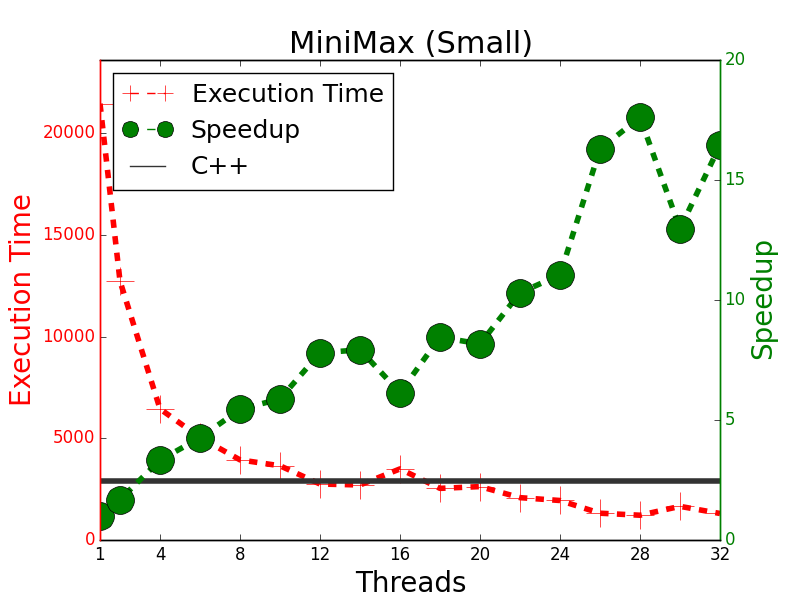
\includegraphics[width=\textwidth]{experiments/scalability/scale-min-max-tictactoe-small.png}
                \label{fig:implementation:scale_minmax_small}
        \end{subfigure}
        ~
        \begin{subfigure}[b]{\plotsize\textwidth}
                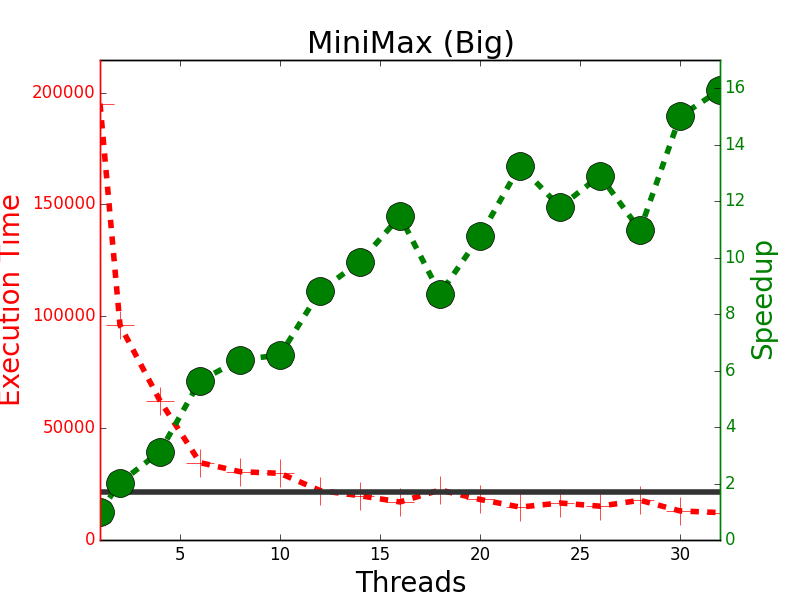
\includegraphics[width=\textwidth]{experiments/scalability/scale-min-max-tictactoe-big.png}
                \label{fig:implementation:scale_minmax_big}
        \end{subfigure}\\

        \caption{Scalability for the MiniMax program. Although the Big
           configuration has more work available and could in principle scale
           better than Small, the high memory requirements of Big makes it scale
           poorly.}

        \label{fig:implementation:scale_minmax}
\end{figure}

The scalability results for the MSSD program are shown in
Fig.~\ref{fig:implementation:scale_sssp}. The amount of work required to compute
the results of each dataset depends on the size of the graph and the number of
nodes from which the distance must be computed. The first conclusion is that
more work implies more scalability, and the US Power Grid dataset has a 20-fold
speedup for 32 threads, the best from the 4 datasets used. The second conclusion is that
all datasets are able to, at least, reach the execution speed of the corresponding
C++ program. However, some datasets such as EU Email, are notoriously faster
than C++ when using more than 5 threads, which is a fairly impressive result. We
think this is because the number of edges, for this particular graph, is almost
equal to the number of nodes. Furthermore, LM as a slight advantage over the C++
program because, in LM, distances to different nodes are propagated at once,
while in the C++ version, the Dijkstra algorithm runs in iterations - one for
each node from which we want to calculate the distance from.

\begin{figure}[]
        \centering
        \begin{subfigure}[b]{\plotsize\textwidth}
                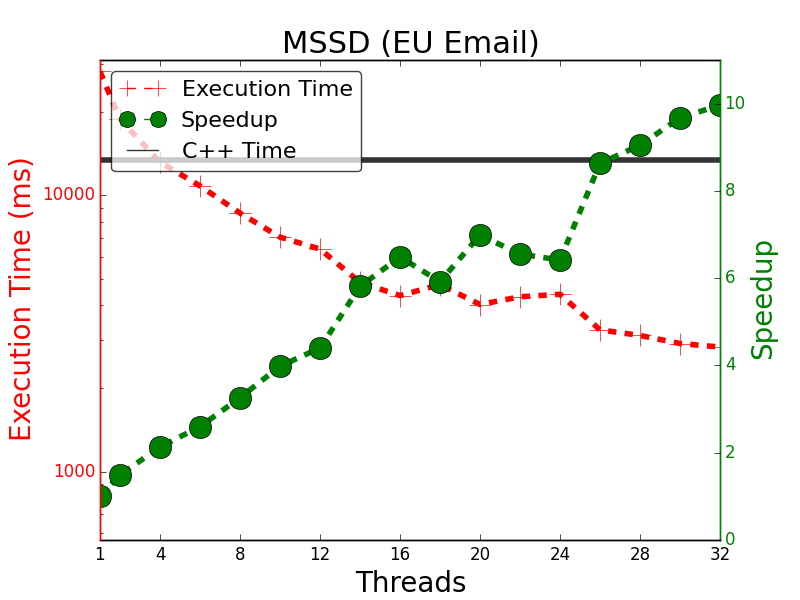
\includegraphics[width=\textwidth]{experiments/scalability/scale-shortest-email.png}
                \label{fig:implementation:scale_sssp_email}
                \caption{Graph with 265000 nodes and 420000 edges. The shortest
                distance is calculated for 100 nodes.}
        \end{subfigure}
        ~
        \begin{subfigure}[b]{\plotsize\textwidth}
                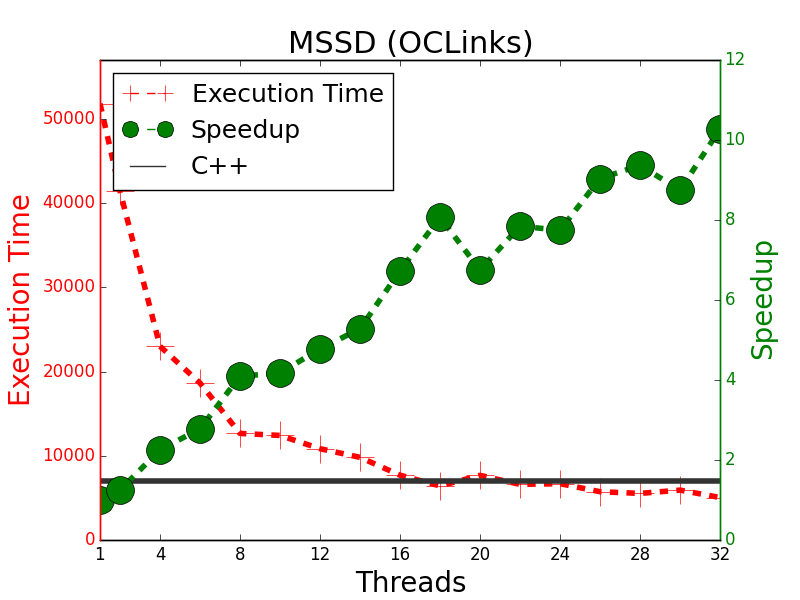
\includegraphics[width=\textwidth]{experiments/scalability/scale-shortest-oclinks.png}
                \label{fig:implementation:scale_sssp_oclinks}
                \caption{Graph with around 2000 nodes and 20000 edges. The shortest
                   distance is calculated for all nodes.}
        \end{subfigure} \\
        \begin{subfigure}[b]{\plotsize\textwidth}
                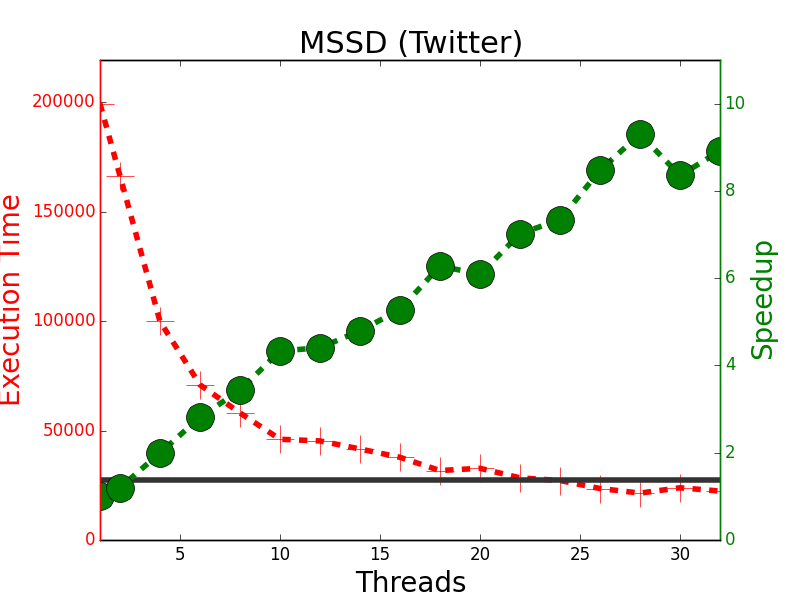
\includegraphics[width=\textwidth]{experiments/scalability/scale-shortest-twitter.png}
                \label{fig:implementation:scale_sssp_twitter}
                \caption{Graph with 81306 nodes and 1768149 edges. The shortest
                   distance is calculuated for 40 nodes.}
        \end{subfigure}
        ~
        \begin{subfigure}[b]{\plotsize\textwidth}
                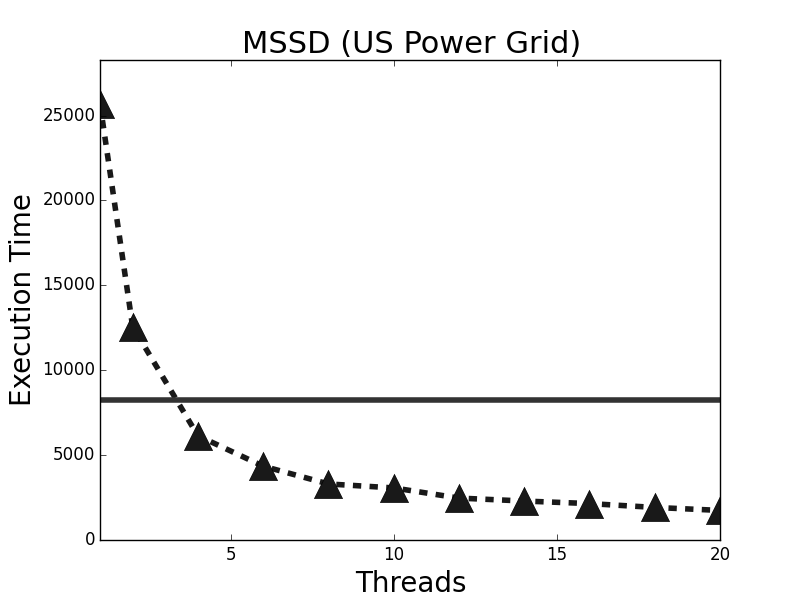
\includegraphics[width=\textwidth]{experiments/scalability/scale-shortest-uspowergrid.png}
                \label{fig:implementation:scale_sssp_uspowergrid}
                \caption{Graph with around 5000 nodes and 13000 edges. The
                shortest distance is calculated for all nodes.}
        \end{subfigure}\\
        \caption{Scalability for the MSSD program. The LM system scales better
        when there is more work to do, with the US Power Grid dataset being the
        most computationally expensive and the one with the best scalability.}
        \label{fig:implementation:scale_sssp}
\end{figure}

The final scalability results are shown for PageRank in
Fig.~\ref{fig:implementation:scale_pagerank}. We used two datasets, Google Plus
and Pokec. Google Plus has 107614 nodes and 13673453 edges, while Pokec has
1632803 nodes and 30622564 edges. Even though Pokec is the larger graph, Google
Plus has a denser graph, where the average number of edges per node is 127
compared to the average of 18 for Pokec. This may explain why Google Plus is
more scalable with a 14-fold speedup for 32 threads.

\begin{figure}[]
        \begin{subfigure}[b]{\plotsize\textwidth}
                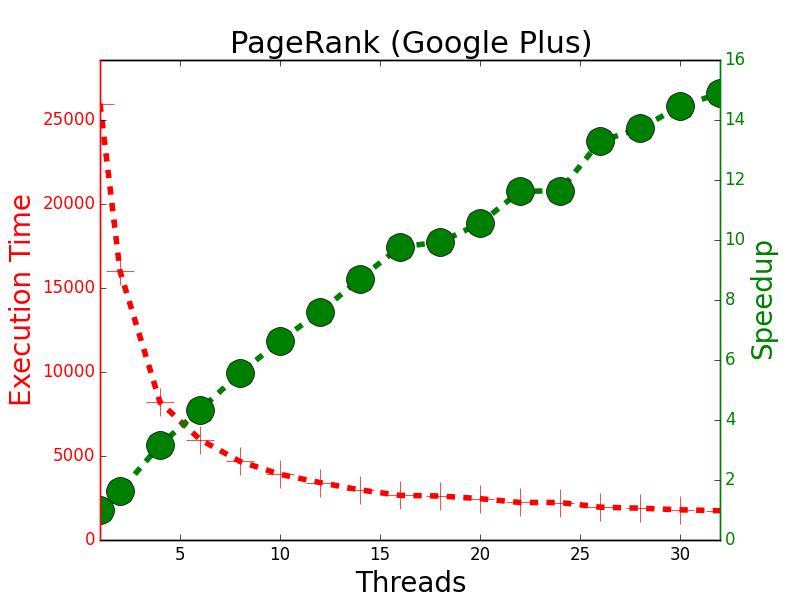
\includegraphics[width=\textwidth]{experiments/scalability/scale-pagerank-gplus.png}
                \label{fig:implementation:scale_pagerank_gplus}
                \caption{The Google Plus graph has a high average of edges per
                node of 127.}
        \end{subfigure}
        ~
        \begin{subfigure}[b]{\plotsize\textwidth}
                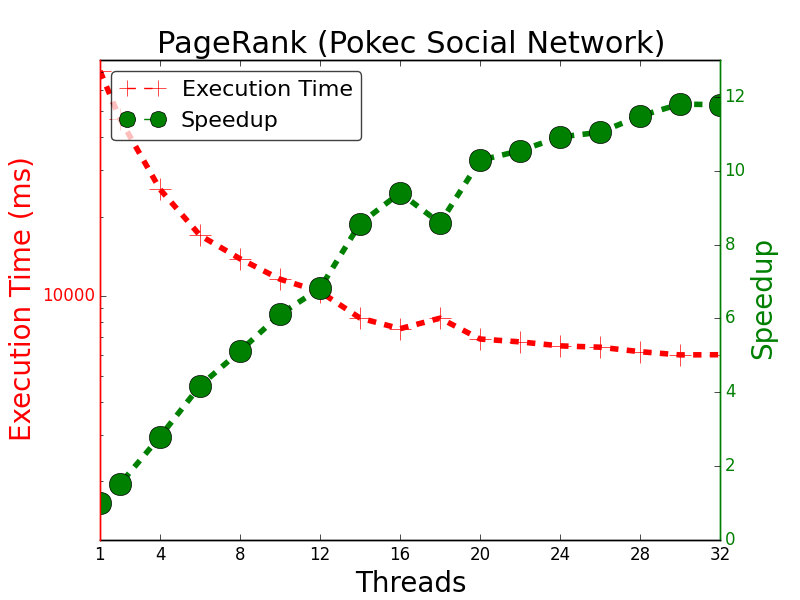
\includegraphics[width=\textwidth]{experiments/scalability/scale-pagerank-pokec.png}
                \label{fig:implementation:scale_pagerank_pokec}
                \caption{The Pokec graph has a lower average of edges per node
                of 18.}
        \end{subfigure}\\
        \caption{Scalability results for the asynchronous PageRank program. The
           superior scalability of the Google Plus dataset may be explained by
        its higher density of edges.}
        \label{fig:implementation:scale_pagerank}
\end{figure}
